
\chapter{Introducción. Propiedades básicas de los fluidos}

\section{Definición de fluido}

Definición corta:


\fbox{\textcolor{red}{\textbf{Material incapaz de resistir esfuerzos tangenciales}}}

\begin{itemize}
	\item \textit{esfuerzo} : Fuerza por unidad de superficie
	
	\item \textit{tangencial} : ni compresión ni dilatación
\end{itemize}


Simplificaci\'on: \textbf{los fluidos son materiales muy f\'acilmente deformables.}

\bigskip

Pero la separaci\'on entre s\'olidos y fluidos no est\'a clara. Hay materiales
que se resiten a una clasificaci\'on sencilla. P.e. : pinturas, pastas, pol\'{\i}meros,
etc ... Ser\'an analizados en detalle en el tema de \textbf{Reolog\'{\i}a.}


A nivel molecular, la diferencia entre l\'{\i}quidos y gases tiene relaci\'on con la magnitud de
la fuerza entre mol\'eculas.


\begin{figure}
	\centering       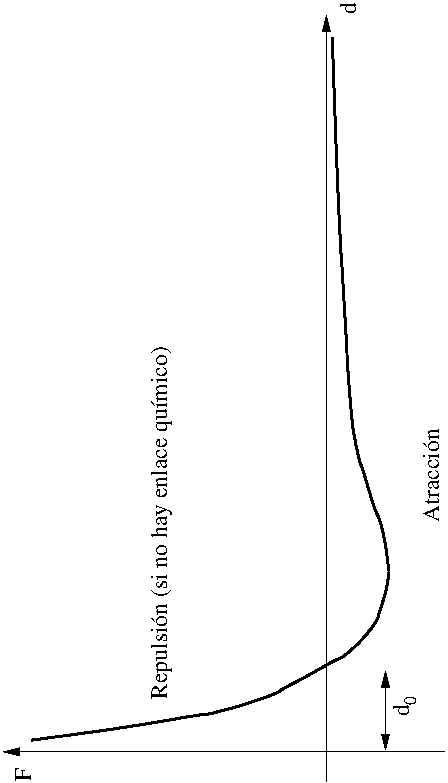
\includegraphics[scale=1,angle=270]{TeX_files/chapter01-Introduccion/fuerzas_molec.pdf}
	\caption{Fuerzas intermoleculares}
	
\end{figure}

En $d_0$, se produce un equilibrio estable.

Para la mayoria de las mol\'eculas, $d_0$ es del orden de  $3-4\cdot10^{-10}$ metros.

Para l\'{\i}quidos, la distancia entre mol\'eculas es, aproximadamente, $d_0$. P.e., para el agua:

$$
\rho \approx 1000 \, \textrm{Kg}/\textrm{m}^3
$$
$$
\textrm{Peso molecular} \approx 0.018 \, \textrm{Kg}/\textrm{mol} \Rightarrow
m = 3.0 \cdot 10^{-26} \, \textrm{Kg}/\textrm{molecula}
$$
$$
V_m = \frac{3.0 \cdot 10^{-26} \, \textrm{Kg}/\textrm{molecula}}{1000 \, \textrm{Kg}/\textrm{m}^3}
=3.0 \cdot 10^{-29} \, \textrm{m}^3
$$
$$
V_m = \frac{4}{3} \pi R^3 \Rightarrow R \approx 1.9 \cdot 10^{-10} \, \textrm{m}
$$

Para los gases, la distancia es mucho mayor (Ejercicio: calcular $d$ para el aire).

As\'{\i}, las fuerzas entre las mol\'eculas de un gas son atractivas y muy d\'ebiles. Estas mol\'eculas
flotan por el espacio sin pr\'acticamente ninguna interacci\'on excepto las colisiones.

\section{Hipótesis del medio continuo}

Todos los materiales est\'an formados por mol\'eculas. Las propiedades del material no estan distribuidas
uniformemente. Si la escala de observaci\'on es lo bastante peque\~na, la composici\'on molecular del material
debe tenerse en cuenta (hablamos entonces de {\em Mec\'anica Estad\'{\i}stica}).

Sin embargo, en {\em Mec\'anica de Fluidos}, se habla normalmente de la densidad, la temperatura, la velocidad,
como una \textcolor{red}{distribuci\'on uniforme de estas propiedades}, sin considerar la naturaleza discreta de la materia. Es
normal hablar de "diferenciales de volumen". Sin embargo, estos diferenciales no son los mismos que los usados
en C\'alculo Infinitesimal. Son volumenes finitos, pero

\begin{itemize}
	\item lo suficientemente grandes como para albergar un n\'umero enorme de mol\'eculas, de forma que las fluctuaciones en las propiedades se anulen entre s\'{\i}, y
	\item lo suficientemente peque\~nos como para que la propiedad pueda ser considerada \em{local}.
\end{itemize}

Batchelor \cite{Bat} lo describe muy bien con una figura parecida a esta:
\begin{center}
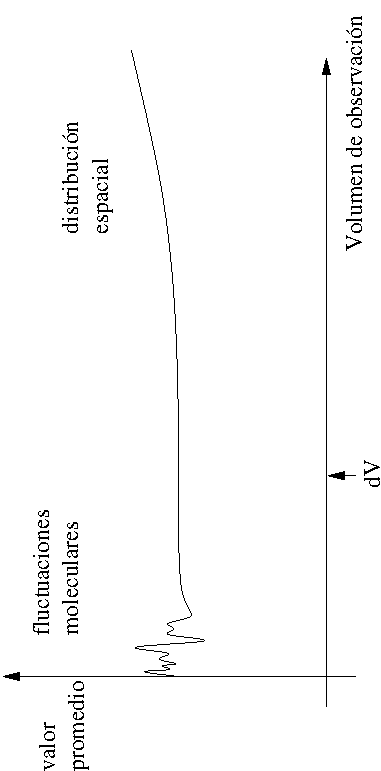
\includegraphics[scale=1,angle=270]{TeX_files/chapter01-Introduccion/difer_vol.pdf}
\end{center}

\section{Propiedades de los fluidos}
\begin{itemize}
	\item \textbf{Propiedades mec\'anicas}
	\begin{itemize}
		\item{\textcolor{red}{densidad - volumen espec\'{\i}fico}}
		$$
		\rho = \frac{m}{V} \qquad ; \qquad \left[\rho\right] = \frac{\textrm{Kg}}{\textrm{m}^3}
		$$
		$$
		v = \frac{1}{\rho} = \frac{V}{m} \qquad ; \qquad \left[v\right] = \frac{\textrm{m}^3}{\textrm{Kg}}
		$$
		\item{\textcolor{red}{M\'odulo de elasticidad} (isot\'ermico)}
		$$
		\beta_T = -v \left(\deriv{p}{v}\right)_T = \rho \left(\deriv{p}{\rho}\right)_T \qquad ; \qquad \left[\beta_T\right] = \textrm{Pa}
		$$
		
		Dado que, \textit{para un gas ideal a temperatura constante}, $\rho \propto p$, tenemos que $\beta_T = p$.
		
		Para una variaci\'on de presi\'on $\Delta p$, la variaci\'on relativa de densidad se puede calcular mediante
		
		$$
		\frac{\Delta \rho}{\rho} = \frac{\Delta p}{\beta_T}
		$$
		
		
		\begin{quotation}
			\textbf{Criterio de compresibilidad} : Todos los fluidos son compresibles, en mayor o menor grado.
			Es importante saber en qu\'e condiciones  un fluido podr\'a ser considerado compresible y cu\'ando no. Supongamos que es considerado compresible si $\frac{\Delta \rho}{\rho} \leq 0.01$. Entonces,
			$$
			\frac{\Delta p}{\beta_T} \lessapprox 0.01.
			$$
			
			Como veremos m\'as adelante, se puede relacionar $\Delta p$ con la velocidad de flujo,
			$$
			\Delta p \sim \frac{1}{2} \rho u^2,
			$$
			de forma que un fluido con velocidad $u$ se puede considerar incompresible si
			$$
			\frac{\rho u^2}{\beta_T} \lessapprox 0.02.
			$$
			
			Como ejemplo, consideremos el aire a presi\'on atmosf\'erica, $ \beta_T = p = 10^5 \,\textrm{Pa}$,
			$\rho \approx 1.2 \,\frac{\textrm{Kg}}{\textrm{m}^3}$.
			
			$$ u^2 \lessapprox \frac{0.02 \beta_T}{\rho} = \frac{0.02 \cdot 10^5}{1.2} = 1.66 \cdot 10^3 \textrm{m}^2/\textrm{s}^2$$
			$$ \Rightarrow u \approx 40 \, \textrm{m/s} $$
			
			\subsection*{Ejercicio} 
			Para el agua, a $20^\circ C$ y presi\'on atmosf\'erica, $\beta_T \approx \unit[2.2\times 10^9]{Pa}$
			y $\rho \approx \unit[1000]{Kg/m^3}$.
			Calcular para qu\'e orden de magnitud de velocidad de flujo el agua debe empezar a considerarse compresible.
		\end{quotation}
		
		\item{\textcolor{red}{Viscosidad}}
		
		Si un fluido fluye en la direcci\'on $x$, de forma ordenada, por capas, aumentando la velocidad en la direcci\'on
		$z$, como muestra la figura,
		
		\begin{center}
			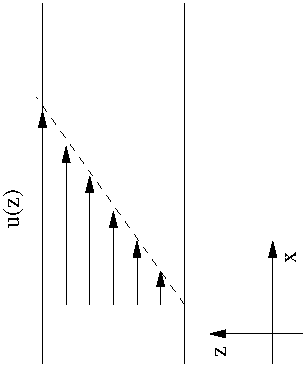
\includegraphics[scale=1,angle=270]{TeX_files/chapter01-Introduccion/u_z.pdf}
		\end{center}
		
		se produce un intercambio de cantidad de movimiento entre capas que tiende a frenar las m\'as r\'apidas y acelerar las m\'as lentas. Es decir, se produce un \textit{esfuerzo tangencial}. En muchos casos, \'este esfuerzo es proporcional al gradiente de velocidades, y a la constante de proporcionalidad se le denomina \textit{\textcolor{red}{viscosidad din\'amica}}, $\mu$. Ésta es la conocida como \textbf{Ley de Newton de la viscosidad}.
		
		\begin{equation}
			\tau = \mu \dparc{u}{z} \qquad ; \qquad \left[\mu\right] = \textrm{Pa}\cdot\textrm{s}
		\end{equation}
		
		
		La \textit{\textcolor{red}{viscosidad cinem\'atica}} se define como
		$$
		\nu = \frac{\mu}{\rho} \qquad ; \qquad \left[\nu\right] = \frac{\textrm{m}^2}{s}
		$$
		
		Ampliaremos el concepto de viscosidad en el tema siguiente.
		
	\end{itemize}
	\item {\textbf{Propiedades termodin\'amicas}}
	
	\textcolor{red}{entalp\'{\i}a}
	$$ h = u + \frac{p}{\rho} = u + p v \qquad ; \qquad \left[h\right] = \left[u\right] = \frac{\textrm{J}}{\textrm{Kg}},
	$$
	
	\textcolor{red}{calor espec\'{\i}fico}
	\begin{eqnarray*}
		c_v = \left(\dparc{q}{T}\right)_v = \dparc{u}{T} & \textrm{a volumen constante} \\
		c_p = \left(\dparc{q}{T}\right)_p = \dparc{h}{T} & \textrm{a presi\'on constante}
	\end{eqnarray*}
	$$
	\left[ c_p \right] = \left[ c_v \right] = \frac{\textrm{J}}{\textrm{Kg}\cdot\textrm{K}}
	$$
	
	La relaci\'on entre ambos coeficientes es:
	$$
	c_p = c_v + \dparc{p v}{T}
	$$
	
	Para un gas perfecto,
	$$ pv = R^\prime T  \Rightarrow \dparc{pv}{T} = R^\prime $$
	$$ \Rightarrow c_p = c_v + R^\prime $$,
	donde $R^\prime = \frac{R}{M}$.
	
	El cociente entre los dos coeficientes se denomina \textit{\textcolor{red}{exponente adiab\'atico}},
	$$
	\gamma = \frac{c_p}{c_v}.
	$$
	
	\textcolor{red}{coeficiente de expansi\'on t\'ermica}
	
	Normalmente,  $\uparrow T \Rightarrow \uparrow v \, (\Rightarrow \downarrow \rho)$.
	
	$$
	\alpha = \frac{1}{v}\deriv{v}{T} = - \frac{1}{\rho} \deriv{\rho}{T} \qquad; \qquad \left[ \alpha \right] = \textrm{K}^{-1}
	$$
	
	Para agua en condiciones normales, $\alpha \approx 1.5\cdot10^{-4} \,\textrm{K}^{-1}$.
	
	Consideremos un gas perfecto, a presi\'on constante,
	$$
	\alpha_p = -\frac{1}{\rho}\left( \dparc{\rho}{T}\right)_p,
	$$
	como $\rho = \frac{p}{R^\prime T}$,
	$$\left(\dparc{\rho}{T}\right)_p = -\frac{p}{R^\prime T^2} \qquad \Rightarrow \alpha_p = \frac{1}{T}$$	
\end{itemize}

\section{Fuerzas sobre fluidos}
\subsection{Fuerzas de superficie}

Act\'uan sobre el contorno de un  volumen determinado de fluido.

Se crean por contacto bien del mismo fluido, un fluido diferente o un s\'olido.

Dada una superficie $\delta \vec S$, y una fuerza superficial $\delta \vec F$ actuando sobre ella, \'esta se
puede descomponer en una componente normal y una componente tangencial.

\begin{center}
	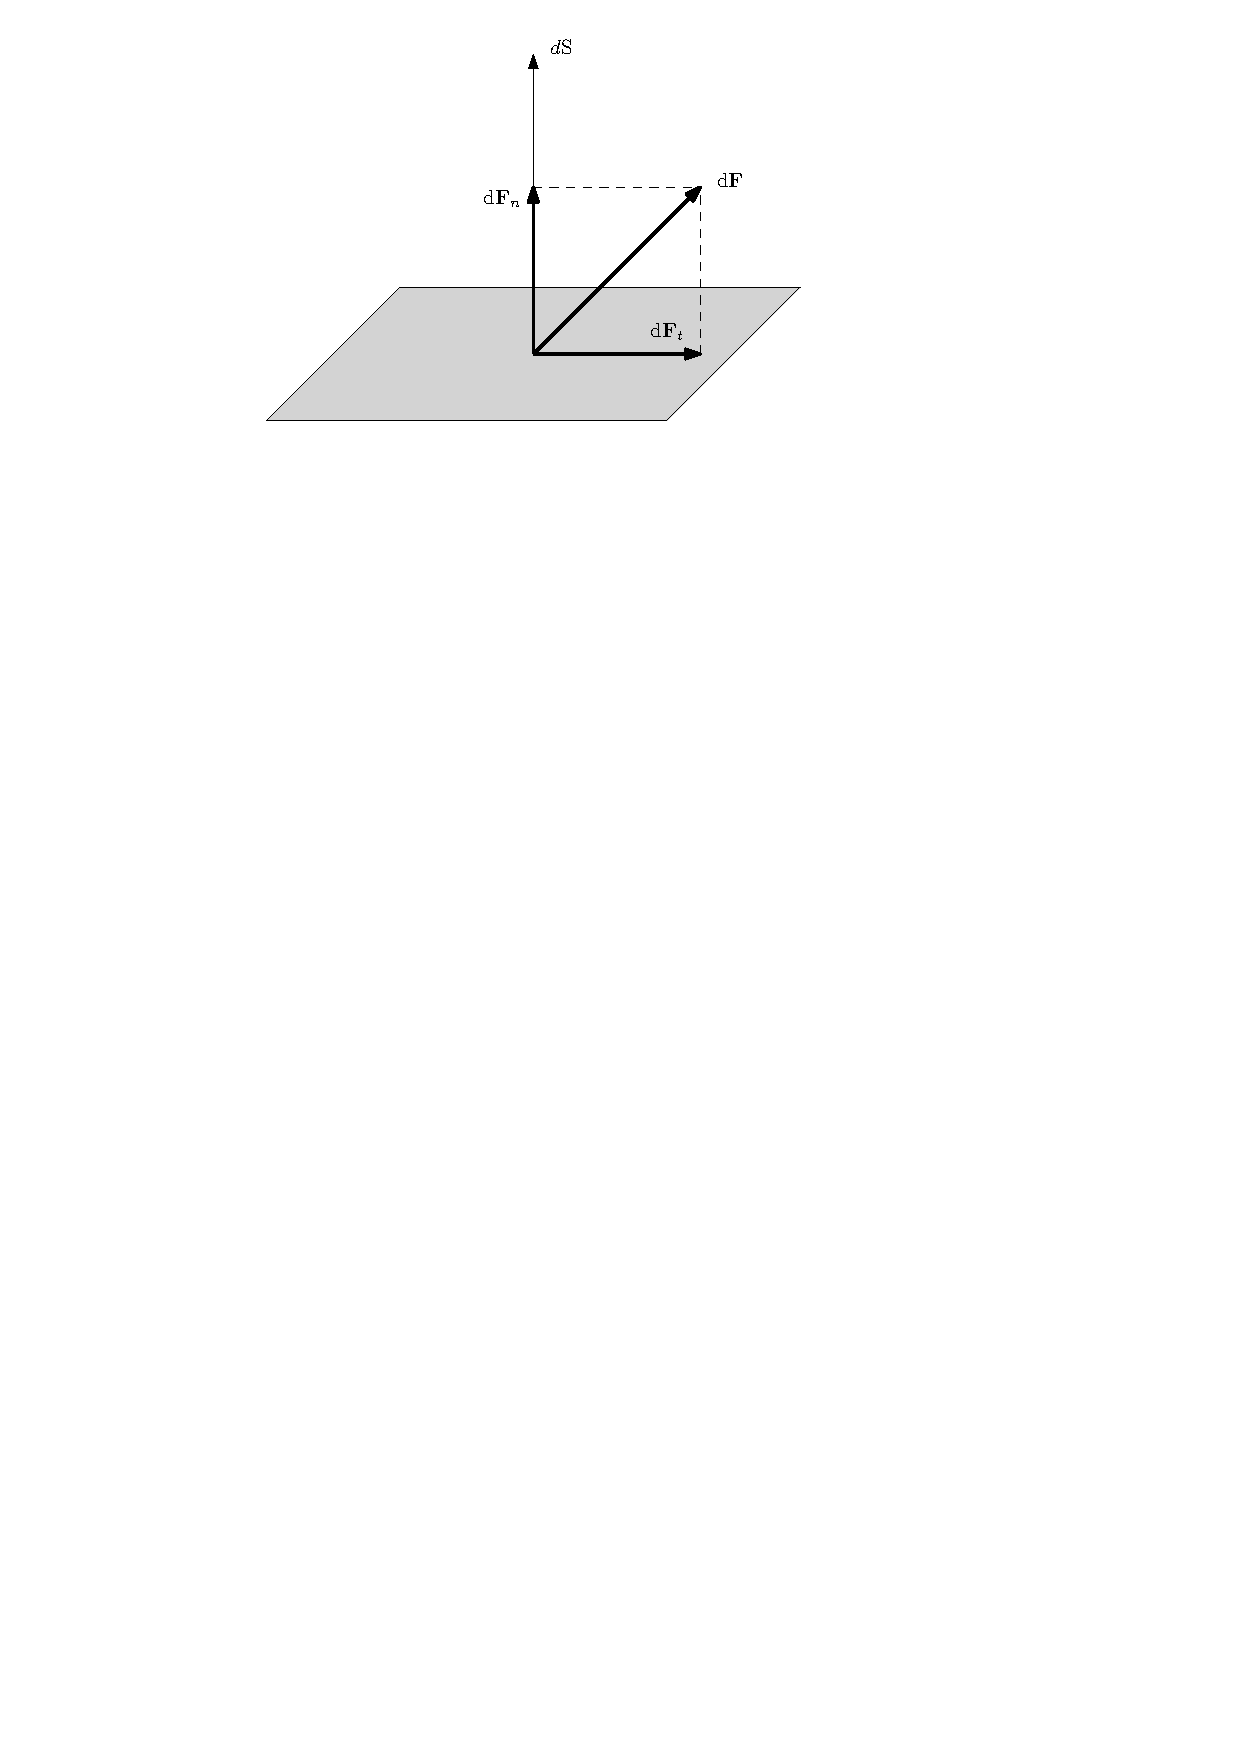
\includegraphics{TeX_files/chapter01-Introduccion/dS.pdf}
\end{center}

Definici\'on de tensi\'on o esfuerzo:

%\begin{center}
	\begin{tabular}{ll}
		\textcolor{blue}{esfuerzo normal} : & \begin{minipage}{10cm}$$\sigma = \lim_{\delta \vec S \rightarrow 0} \frac{\delta \vec F_n}{\delta \vec S}$$\end{minipage} \\
		\textcolor{blue}{esfuerzo tangencial} : & \begin{minipage}{10cm}$$\tau = \lim_{\delta \vec S \rightarrow 0} \frac{\delta \vec F_t}{\delta \vec S}$$ \end{minipage}\\
	\end{tabular}
%\end{center}

\begin{description}
	\item[$\sigma_i$ :] esfuerzo normal aplicado sobre una superficie normal al eje $i$ (y, por lo tanto, paralelo al eje $i$)
	\item[$\tau_{ij}$ :] esfuerzo tangencial aplicado sobre una superficie normal al eje $i$, y en la direcci\'on del eje $j$
\end{description} 

\begin{center}
%	\tikzstyle{isometric}=[x={(0.710cm,-0.410cm)},y={(0cm,0.820cm)},z={(-0.710cm,-0.410cm)}]
\tikzstyle{dimetric} =[x={(0.935cm,-0.118cm)},y={(0cm,0.943cm)},z={(-0.354cm,-0.312cm)}]
\tikzstyle{dimetric2}=[x={(0.935cm,-0.118cm)},z={(0cm,0.943cm)},y={(+0.354cm,+0.312cm)}]
\tikzstyle{trimetric}=[x={(-0.926cm,0.207cm)},y={(0cm,0.837cm)},z={(0.378cm,0.507cm)}]

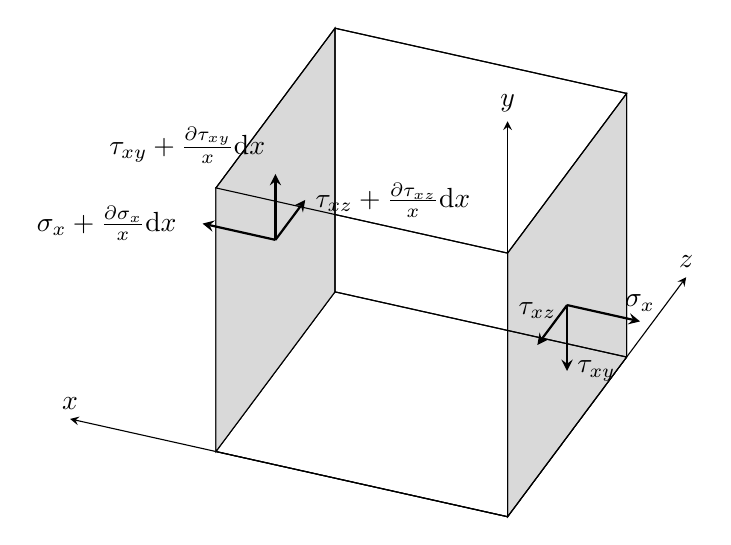
\begin{tikzpicture}[trimetric]
	\coordinate (O) at (0,0,0);
	\draw[-stealth] (0,0,0) -- (6,0,0) node[above]{$x$};
	\draw[-stealth] (0,0,0) -- (0,6,0) node[above]{$y$};
	\draw[-stealth] (0,0,0) -- (0,0,6) node[above]{$z$};
	\draw[fill=gray!30] (0,0,0) -- (0,4,0) -- (0,4,4) -- (0,0,4)-- cycle;	
	\draw (0,0,0) -- (4,0,0) -- (4,4,0) -- (0,4,0)-- cycle;
	\draw (0,0,0) -- (0,0,4) -- (4,0,4) -- (4,0,0)-- cycle;
	\draw[fill=gray!30] (4,0,0) -- (4,4,0) -- (4,4,4) -- (4,0,4)-- cycle;	
	\draw (0,0,4) -- (4,0,4) -- (4,4,4) -- (0,4,4)-- cycle;
	\draw (0,4,0) -- (0,4,4) -- (4,4,4) -- (4,4,0)-- cycle;
%
	\draw[-stealth,thick] (0,2,2) -- (-1,2,2) node[above ]{$\sigma_x$};
	\draw[-stealth,thick] (0,2,2) -- (0,1,2) node[right]{$\tau_{xy}$};
	\draw[-stealth,thick] (0,2,2) -- (0,2,1) node[above=2mm]{$\tau_{xz}$};
%
	\draw[-stealth,thick] (4,2,2) -- (5,2,2) node[left=2mm]
					{$\sigma_x+\frac{\partial \sigma_x}{x} \textrm{d}x$};
	\draw[-stealth,thick] (4,2,2) -- (4,3,2) node[above left]
					{$\tau_{xy}+\frac{\partial \tau_{xy}}{x} \textrm{d}x$};
	\draw[-stealth,thick] (4,2,2) -- (4,2,3) node[right]
					{$\tau_{xz}+\frac{\partial \tau_{xz}}{x} \textrm{d}x$};
\end{tikzpicture}
\tikzstyle{isometric}=[x={(0.710cm,-0.410cm)},y={(0cm,0.820cm)},z={(-0.710cm,-0.410cm)}]
\tikzstyle{dimetric} =[x={(0.935cm,-0.118cm)},y={(0cm,0.943cm)},z={(-0.354cm,-0.312cm)}]
\tikzstyle{dimetric2}=[x={(0.935cm,-0.118cm)},z={(0cm,0.943cm)},y={(+0.354cm,+0.312cm)}]
\tikzstyle{trimetric}=[x={(-0.926cm,0.207cm)},y={(0cm,0.837cm)},z={(0.378cm,0.507cm)}]

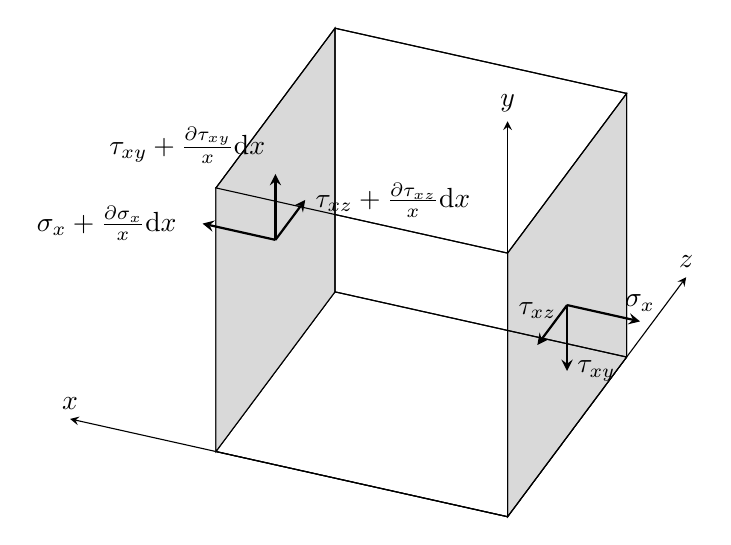
\begin{tikzpicture}[trimetric]
	\coordinate (O) at (0,0,0);
	\draw[-stealth] (0,0,0) -- (6,0,0) node[above]{$x$};
	\draw[-stealth] (0,0,0) -- (0,6,0) node[above]{$y$};
	\draw[-stealth] (0,0,0) -- (0,0,6) node[above]{$z$};
	\draw[fill=gray!30] (0,0,0) -- (0,4,0) -- (0,4,4) -- (0,0,4)-- cycle;	
	\draw (0,0,0) -- (4,0,0) -- (4,4,0) -- (0,4,0)-- cycle;
	\draw (0,0,0) -- (0,0,4) -- (4,0,4) -- (4,0,0)-- cycle;
	\draw[fill=gray!30] (4,0,0) -- (4,4,0) -- (4,4,4) -- (4,0,4)-- cycle;	
	\draw (0,0,4) -- (4,0,4) -- (4,4,4) -- (0,4,4)-- cycle;
	\draw (0,4,0) -- (0,4,4) -- (4,4,4) -- (4,4,0)-- cycle;
%
	\draw[-stealth,thick] (0,2,2) -- (-1,2,2) node[above ]{$\sigma_x$};
	\draw[-stealth,thick] (0,2,2) -- (0,1,2) node[right]{$\tau_{xy}$};
	\draw[-stealth,thick] (0,2,2) -- (0,2,1) node[above=2mm]{$\tau_{xz}$};
%
	\draw[-stealth,thick] (4,2,2) -- (5,2,2) node[left=2mm]
					{$\sigma_x+\frac{\partial \sigma_x}{x} \textrm{d}x$};
	\draw[-stealth,thick] (4,2,2) -- (4,3,2) node[above left]
					{$\tau_{xy}+\frac{\partial \tau_{xy}}{x} \textrm{d}x$};
	\draw[-stealth,thick] (4,2,2) -- (4,2,3) node[right]
					{$\tau_{xz}+\frac{\partial \tau_{xz}}{x} \textrm{d}x$};
\end{tikzpicture}
\end{center}

Sobre el volumen $\text{d} V$ act\'ua una fuerza, debida a los esfuerzos superficiales cuya componente $x$ es
\begin{multline}
	\dif F_x = -\sigma_x  \dif y \dif z + \left(\sigma_x + \dparc{\sigma_x}{x} \dif x\right) \dif y \dif z - \tau_{yx} \dif x \dif z + \left(\tau_{yx} + \dparc{\tau_{yx}}{y}\right) \dif x \dif z \\
	- \tau_{zx} \dif x \dif y + \left(\tau_{zx} + \dparc{\tau_{zx}}{z}\right) \dif x \dif y
	= \dparc{\sigma_x}{x} \dif x \dif y \dif z + \dparc{\tau_{yx}}{y} \dif x \dif y \dif z + \dparc{\tau_{zx}}{z}
	\dif x \dif y \dif z
\end{multline}
De la misma forma:
\begin{eqnarray}
	\dif F_y = \dparc{\sigma_y}{y} \dif x \dif y \dif z + \dparc{\tau_{xy}}{x} \dif x \dif y \dif z + \dparc{\tau_{zy}}{z} \dif x \dif y \dif z \\
	\dif F_z = \dparc{\sigma_z}{z} \dif x \dif y \dif z + \dparc{\tau_{xz}}{x} \dif x \dif y \dif z + \dparc{\tau_{yz}}{y} \dif x \dif y \dif z
\end{eqnarray}

La fuerza por unidad de volumen, debida a los esfuerzos superficiales es entonces
\begin{eqnarray*}
	\vec f = \deriv{\vec F}{V} = \left( \dparc{\sigma_x}{x} + \dparc{\tau_{yx}}{y} + \dparc{\tau_{zx}}{z}\right) \vec \imath \\
	+ \left( \dparc{\tau_{xy}}{x} + \dparc{\sigma_y}{y} +  \dparc{\tau_{zy}}{z} \right) \vec \jmath \\
	+ \left( \dparc{\tau_{xz}}{x}  +  \dparc{\tau_{yz}}{y} + \dparc{\sigma_z}{z} \right) \vec k
\end{eqnarray*}
que se expresa de forma abreviada como
\begin{equation}
	 \vec f = \vec \nabla \vec {\vec \tau}
\end{equation}
donde $\vec {\vec \tau}$ es el \textcolor{red}{tensor de tensiones} (stress tensor)
\begin{equation}
	\vec{\vec{\tau}} =
	\left(
	\begin{array}{ccc}
		\sigma_x & \tau_{xy} & \tau_{xz} \\
		\tau_{yx} & \sigma_y & \tau_{yz} \\
		\tau_{zx} & \tau_{zy} & \sigma_z
	\end{array}\right)
\end{equation}

\subsection{Fuerzas m\'asicas}
Act\'uan a distancia

Son debidas a campos de fuerza (gravitacional, electromagn\'etico, \ldots)

Fluido el\'ectricamente cargado : plasma
\begin{itemize}
	\item Electrohidrodin\'amica
	\item Magnetohidrodin\'amica
\end{itemize}

Caso m\'as com\'un: s\'olo campo gravitacional
$$\vec f_g = \rho \vec g$$

\subsection{Fuerzas lineales (tensi\'on superficial)}
En la interfase de separaci\'on entre dos l\'iquidos reside una cantidad de energ\'{\i}a, correspondiente
a la interacci\'on entre moleculas muy pr\'oximas a la superficie de separaci\'on

Esta energ\'{\i}a es proporcional al \'area de la interfase.
\begin{equation}
	 E_s = \sigma S
\end{equation} 

El par\'ametro $\sigma$ recibe el nombre de \textcolor{blue}{tensi\'on superficial} y tiene unidades de fuerza por
unidad de longitud. Esta fuerza es tangente a la superficie, y normal a la l\'{\i}nea de aplicaci\'on.

El valor de $\sigma$ depende de la naturaleza de los materiales que separa la interfase y de su estado termodin\'amico.

P.e. para la interfase entre agua y aire a $20^\circ C$, $\sigma~=~72.8\cdot10^{-3}~\text{N/m}$


\begin{center}
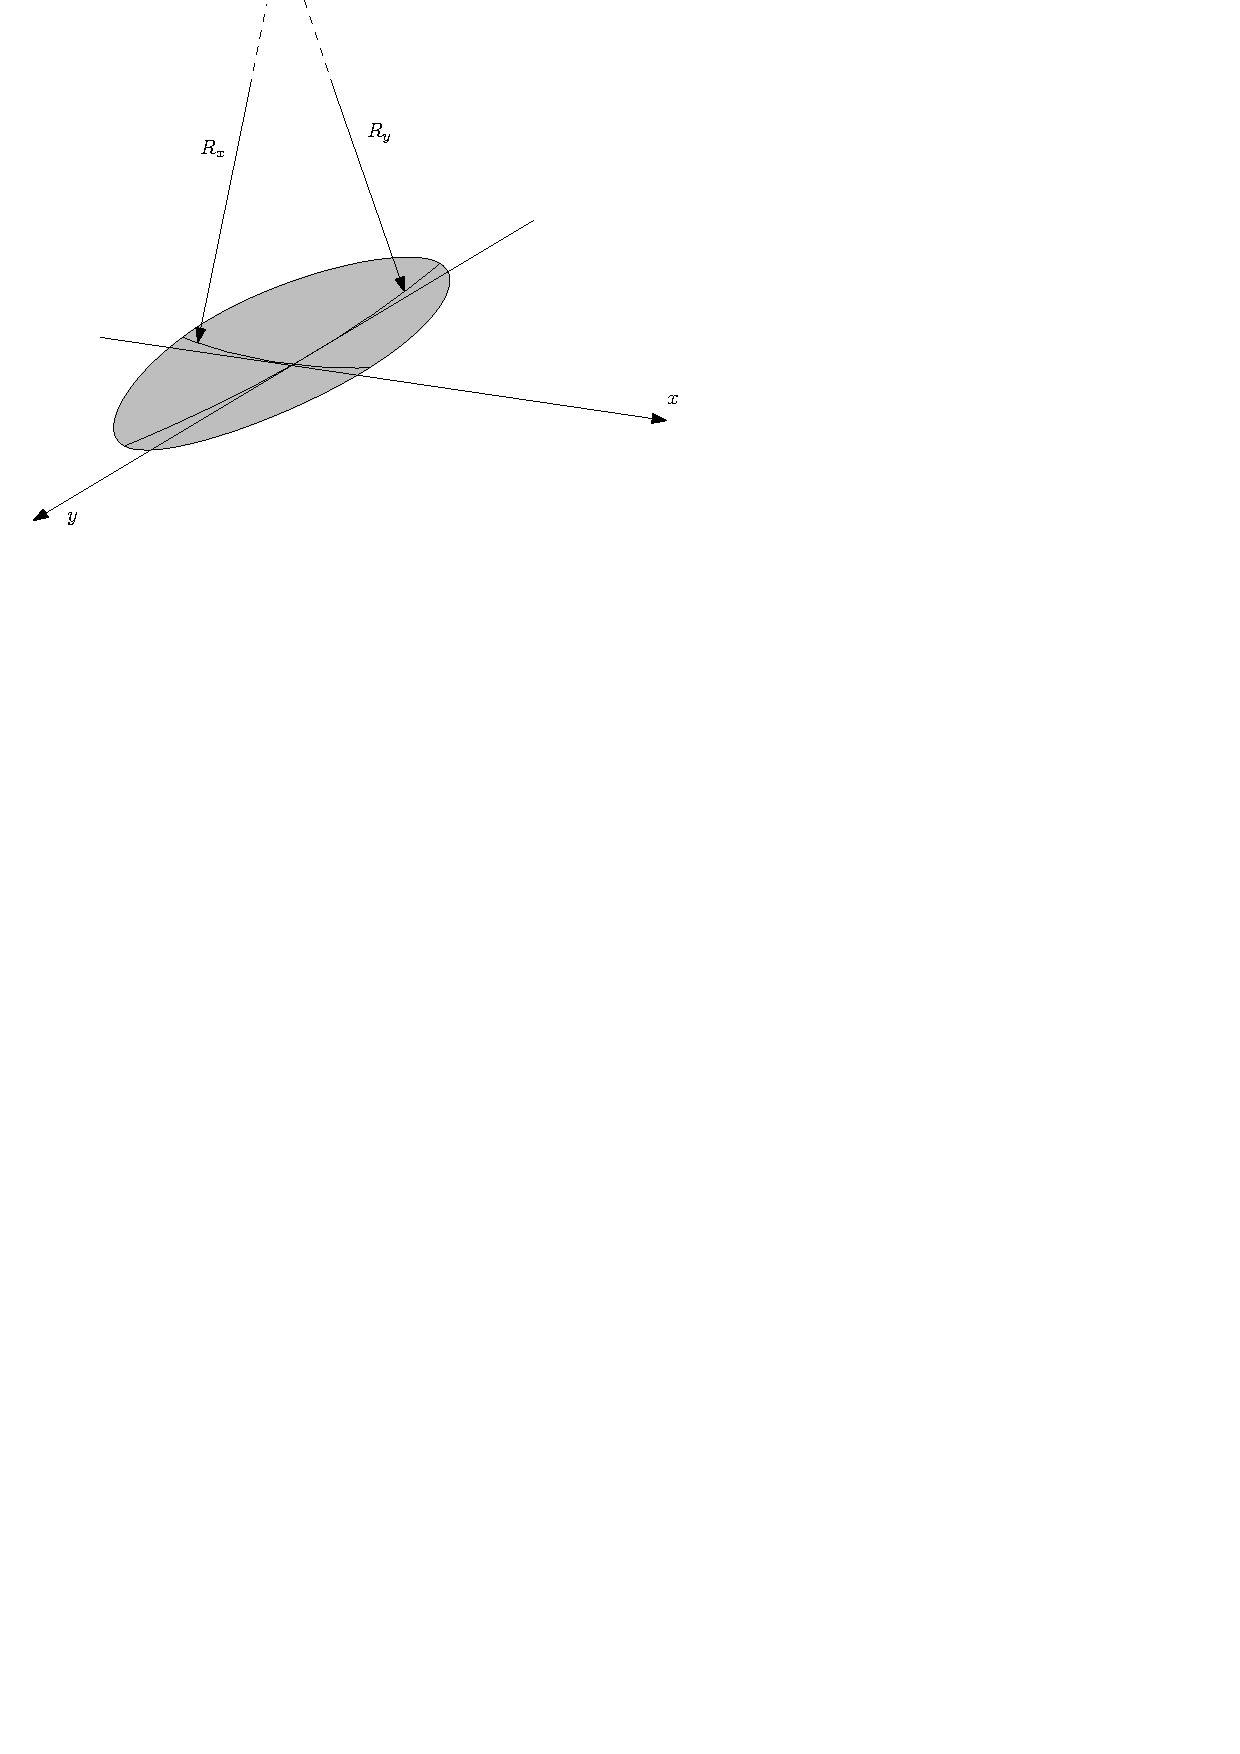
\includegraphics{TeX_files/chapter01-Introduccion/YoungLaplace}
\end{center}
Se puede demostrar (ver \cite{Bat}) que la tensi\'on provocada en la superfice es equivalente a una diferencia
de presi\'on, como indica la \href{https://es.wikipedia.org/wiki/Ley_de_Laplace}{\textbf{ley de Young-Laplace}}
\begin{equation}
	\Delta p = \sigma\left(\frac{1}{R_x}+\frac{1}{R_y}\right)
\end{equation}


Si los dos radios de curvatura son iguales, ($R_x=R_y=R$, casquete esférico), esta expresión se reduce a 
 
\begin{equation}
	\Delta p = \frac{2\sigma}{R}
\end{equation}

Consideramos el caso de tres fluidos (p.e. una gota de aceite en una superficie de agua)
\begin{center}
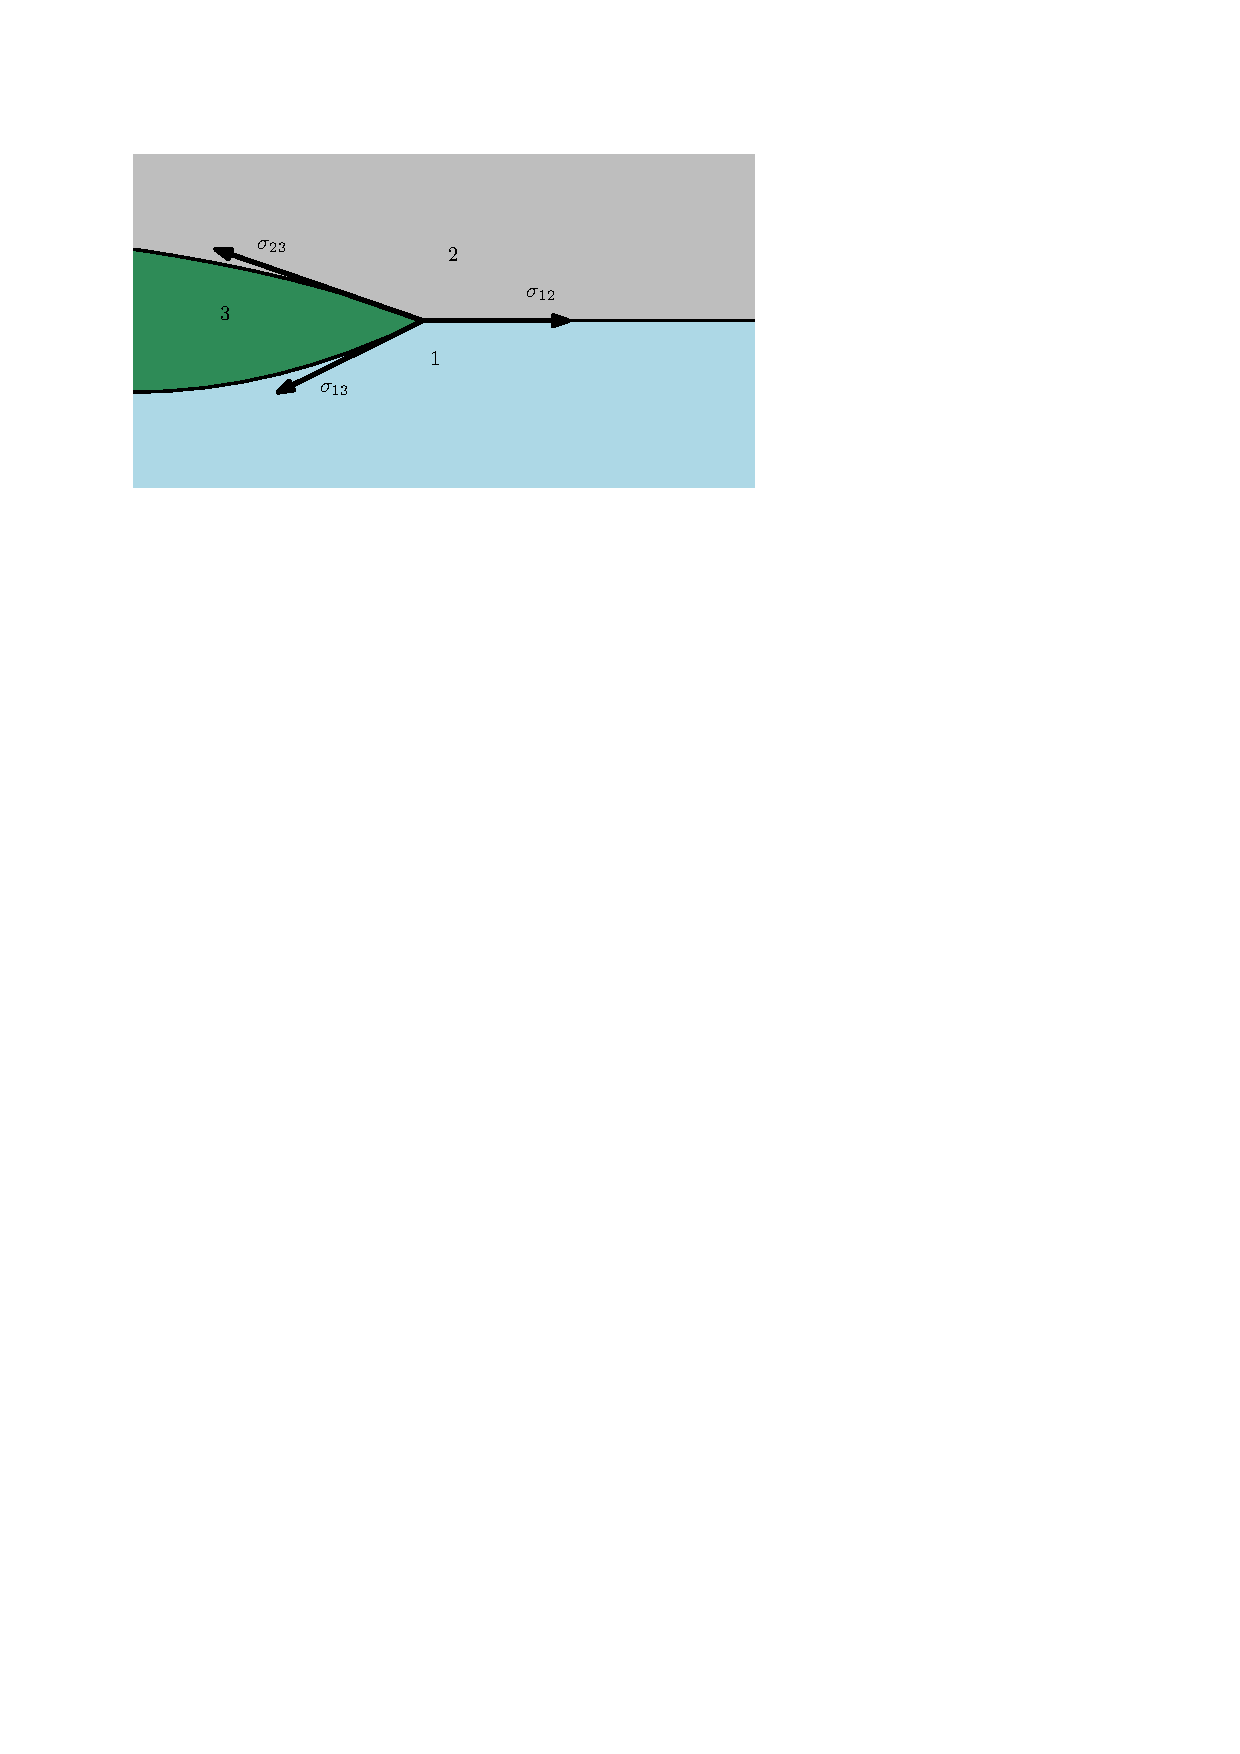
\includegraphics{TeX_files/chapter01-Introduccion/tresFluidos}
\end{center}
Si el m\'odulo de una de las tensiones es mayor que la suma de los m\'odulos de las otras dos, este sistema nunca
puede llegar al equilibrio, y el fluido se expandir\'a de forma indefinida hasta llegar al equilibrio, o tener
un grosor de tama\~no molecular.

Si uno de los materiales es un s\'olido,
\begin{center}
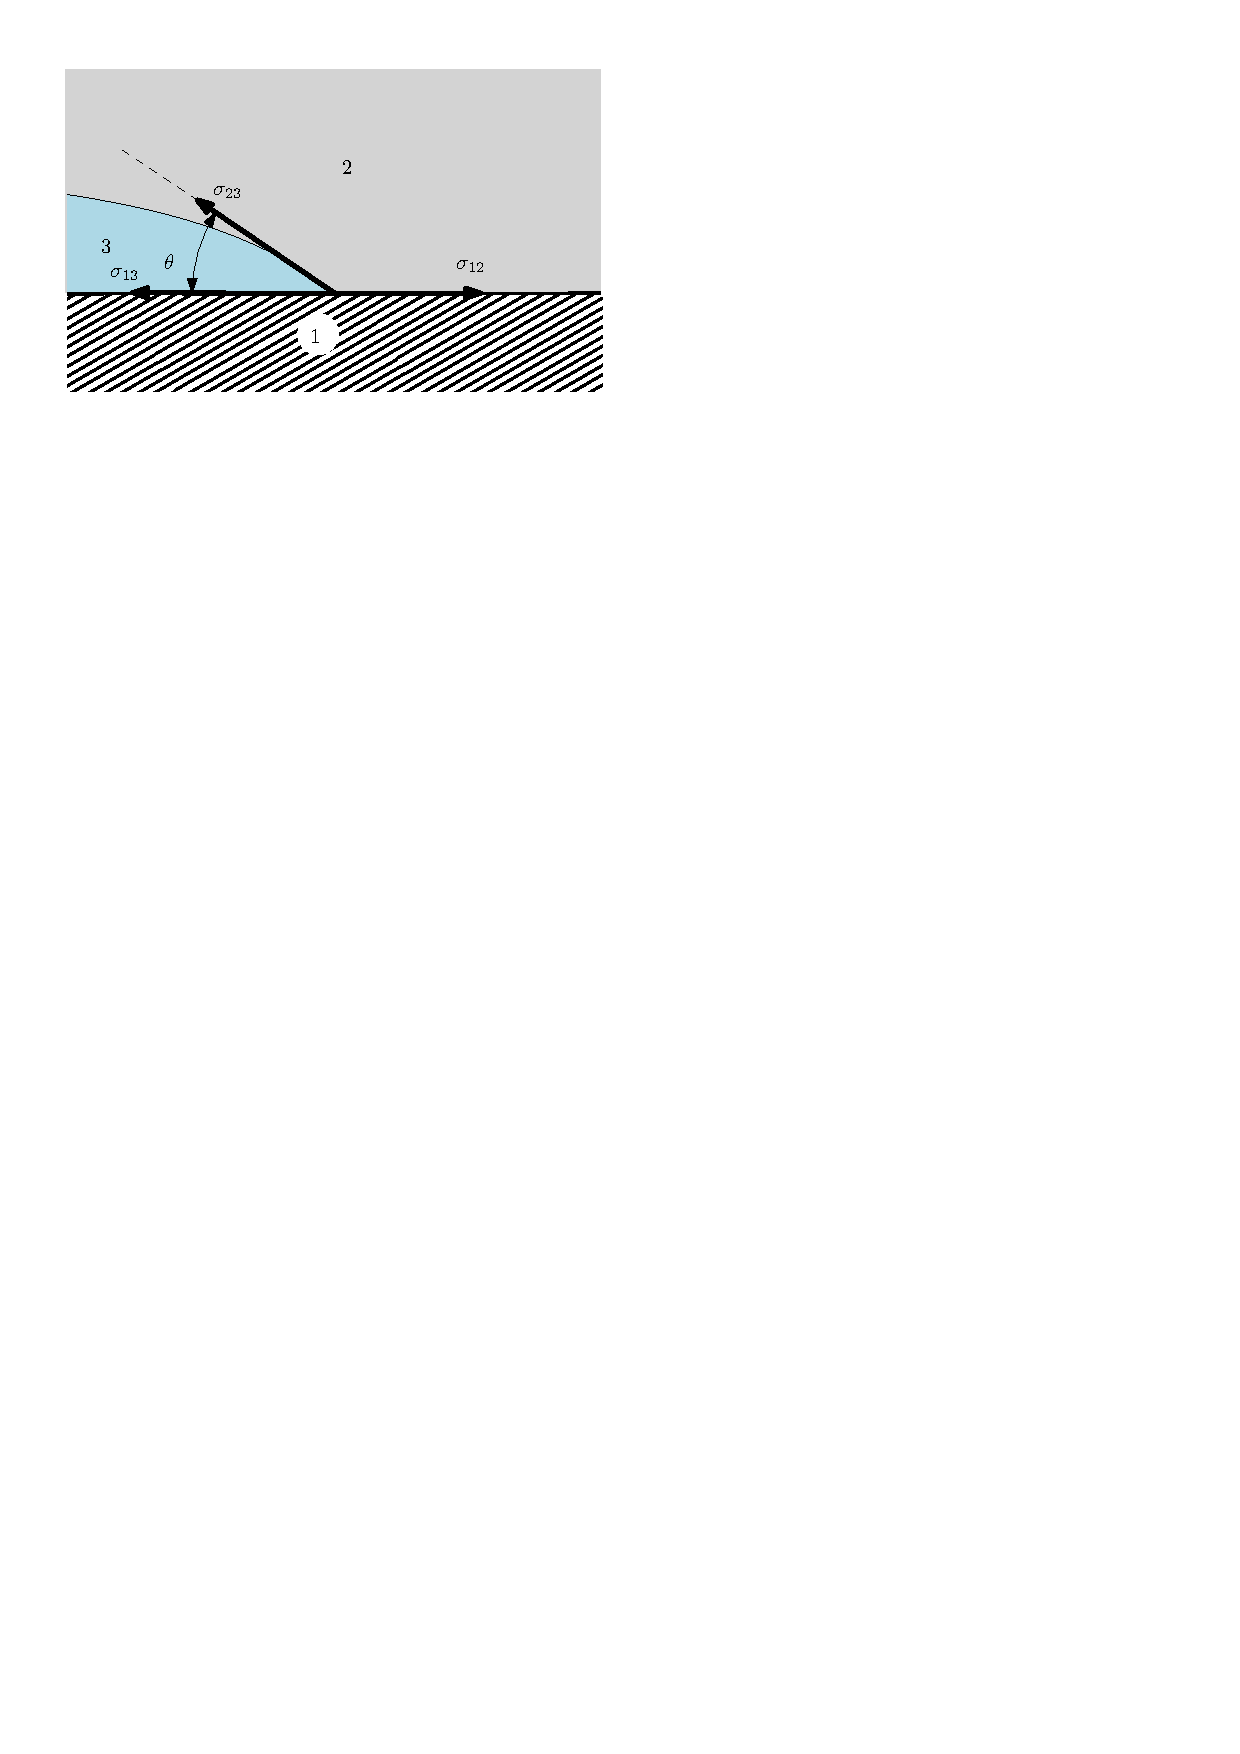
\includegraphics{TeX_files/chapter01-Introduccion/dosysolido}
\end{center}
se llega al equilibrio para
$$ \sigma_{12} = \sigma_{31} + \sigma_{23} \cos{\theta}$$
Se considera que cuanto menor es $\theta$, m\'as "moja" el fluido sobre la superficie del s\'olido.

\subsection*{Ejemplo:}
L\'{\i}quido en contacto con pared plana vertical
\begin{center}
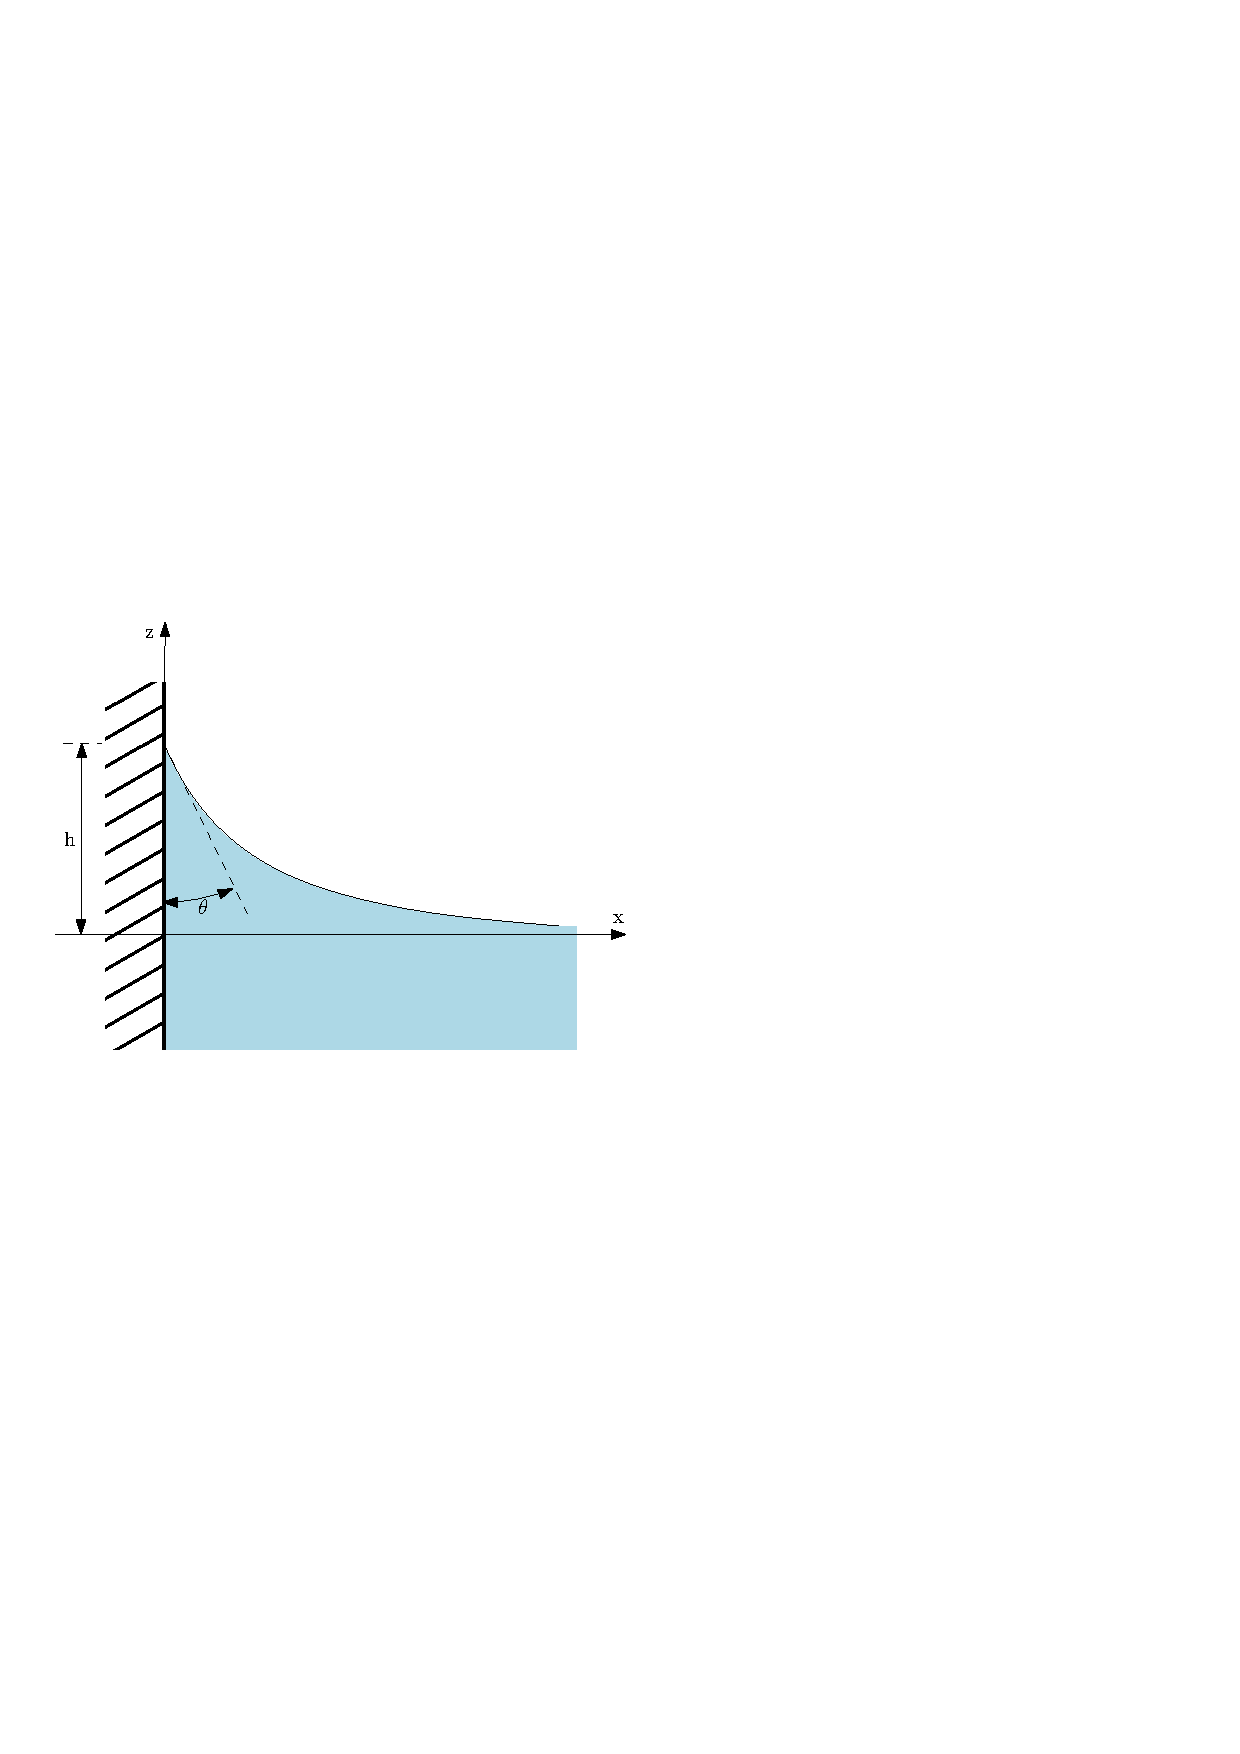
\includegraphics{TeX_files/chapter01-Introduccion/pared.pdf}
\end{center}
Forma de la interficie: $z=\zeta(x)$

En un cierto punto de la interficie, la tensi\'on superficial tiene que ser tal que compense la presi\'on de la columna de fluido. Como veremos m\'as adelante, esta es $\rho g z$, de forma que
$$
\rho g z = \sigma \frac{1}{R_1}
$$
$$
\rho g \zeta = \sigma \frac{\zeta''}{\left( 1 + \zeta'^2\right)^\frac{3}{2}}
$$
Integrando se obtiene
$$
\frac{1}{2}\frac{\rho g}{\sigma}\zeta^2 + \frac{1}{\left(1+\zeta'^2\right)^\frac{1}{2}} = K
$$
Muy lejos de la pared, se cumple que $\zeta=\zeta'=0$, de forma que $K = 1$

Por otro lado, en $x=0$, se tiene (ver figura) $\zeta=h$ y $\zeta'=-\frac{1}{\tan \theta}$, de forma que
$$
h = d \sqrt{2\left(1-\sin \theta \right)}
$$
donde $d^2=\frac{\sigma}{\rho g}$.